\begin{enumerate}[label=\thesection.\arabic{subsection}.\arabic{enumi},ref=\arabic{enumi},leftmargin=4mm,itemsep=9pt]
\item \label{question:C12-Q01}\label{question-short:C12-Q01} Find a vector of magnitude $\sqrt{171}$ perpendicular to both $\vec a=\myvec{1\\-2\\-3}$ and $\vec b=\myvec{3\\-1\\-2}$.
\engsolution
Perpendicularity requires a vector in the null space of the matrix with rows $\vec a^T$ and $\vec b^T$:
\formulausedplain{M=\myvec{1&-2&-3\\3&-1&-2}.}
\formulausedplain{M\vec d=0.}
The two rows are independent, so rank--nullity gives a one-dimensional null space. Its antisymmetric cross-product basis is
\formulaused{\operatorname{Null}(M)=\{\vec v:M\vec v=0\}.}{C12-Q01}
\formulausedplain{\vec a\times\vec b=\myvec{1\\-7\\5}.}
Indeed,
\formulausedplain{\vec a\cdot(1,-7,5)=1+14-15=0.}
\formulausedplain{\vec b\cdot(1,-7,5)=3+7-10=0.}
Every admissible vector is therefore $\vec d=t(1,-7,5)^T$. Since
\formulausedplain{
\|(1,-7,5)\|^2=1+49+25=75,
}
the magnitude condition gives $75t^2=171$, or $t=\pm\sqrt{57}/5$. Hence
\formulausedplain{
\vec d=\pm\frac{\sqrt{57}}5\myvec{1\\-7\\5}.
}
\begin{figure}[H]\centering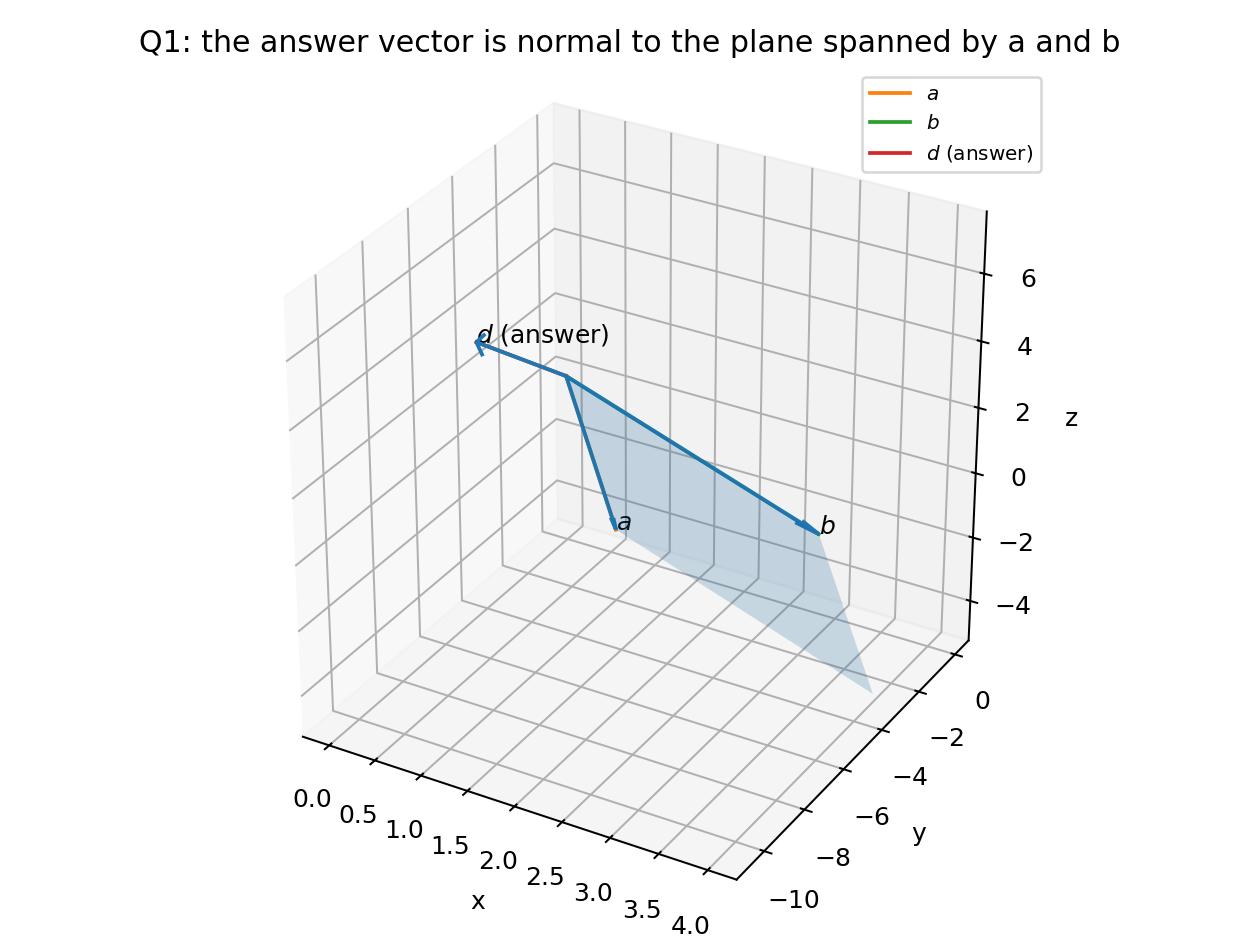
\includegraphics[width=0.96\linewidth]{figs/C12/Q01.png}\end{figure}
\par\smallskip\noindent\textbf{Code reference -}\par\noindent\fbox{\parbox{\dimexpr\linewidth-2\fboxsep-2\fboxrule\relax}{\centering\texttt{codes/C12/Q01.py}}}

\item \label{question:C12-Q05}\label{question-short:C12-Q05} Let $\vec a=\myvec{1\\4\\2}$, $\vec b=\myvec{3\\-2\\7}$ and $\vec c=\myvec{2\\-1\\4}$. Find $\vec d$ perpendicular to both $\vec a,\vec b$ with $\vec c\cdot\vec d=27$.
\engsolution
The antisymmetric bilinear operation supplies a direction perpendicular to both prescribed vectors. Computing its determinant gives
\formulaused{\vec d=t(\vec a\times\vec b)}{C12-Q05}
\formulausedplain{\vec a\times\vec b=\myvec{32\\-1\\-14}.}
Thus the complete perpendicular family is
\formulausedplain{
\vec d=t\myvec{32\\-1\\-14}.
}
The remaining scalar constraint selects the scale. First,
\formulausedplain{
\vec c\cdot(32,-1,-14)=2(32)+(-1)(-1)+4(-14)=64+1-56=9.
}
Therefore $9t=27$, so $t=3$ and
\formulausedplain{
\vec d=\myvec{96\\-3\\-42}.
}
The dot products $\vec a\cdot\vec d=0$ and $\vec b\cdot\vec d=0$, together with $\vec c\cdot\vec d=27$, verify the corrected result.
\begin{figure}[H]\centering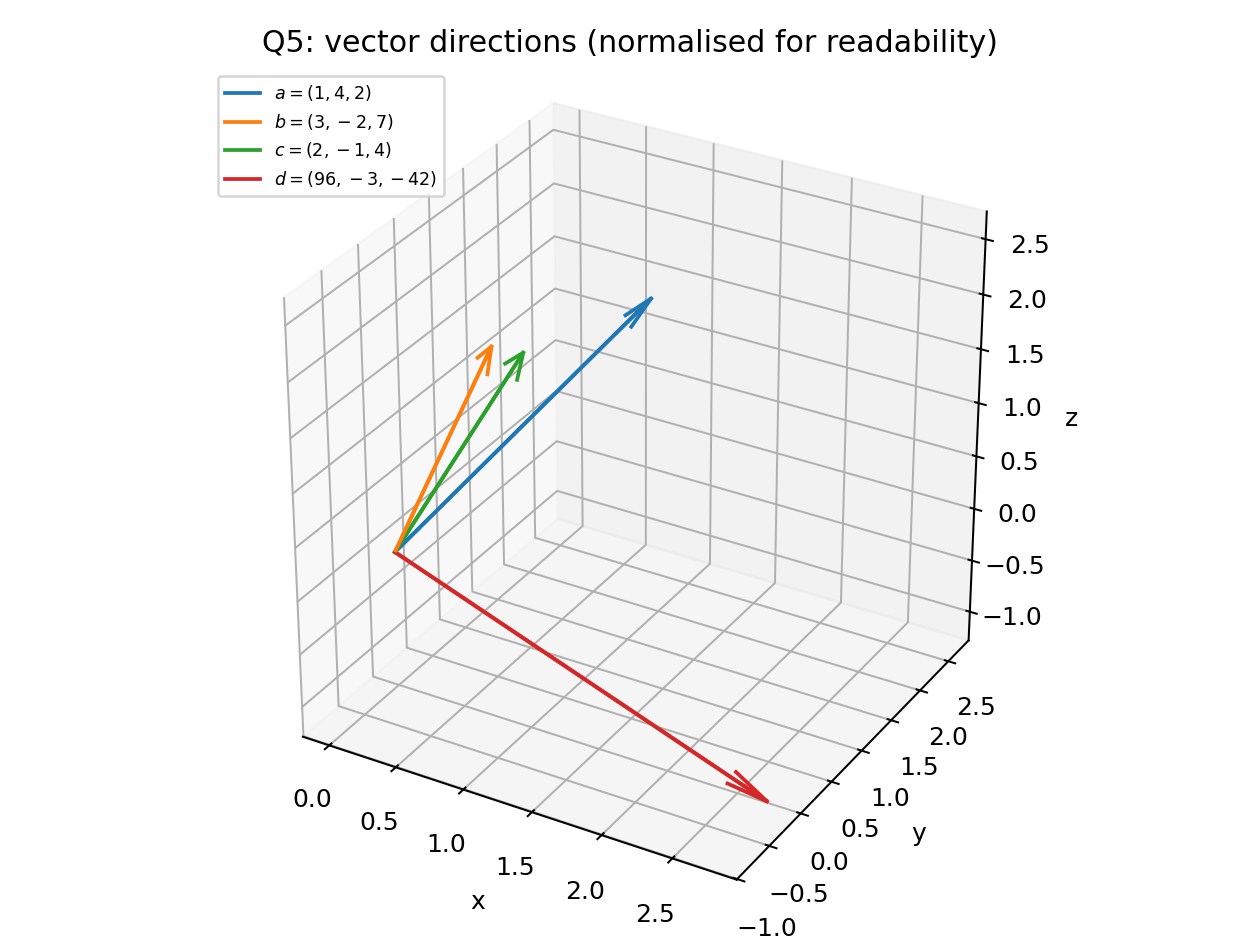
\includegraphics[width=0.96\linewidth]{figs/C12/Q05.png}\end{figure}
\par\smallskip\noindent\textbf{Code reference -}\par\noindent\fbox{\parbox{\dimexpr\linewidth-2\fboxsep-2\fboxrule\relax}{\centering\texttt{codes/C12/Q05.py}}}

\item \label{question:C12-Q06}\label{question-short:C12-Q06} Find the shortest distance between $\vec r=(1,2,3)+\lambda(2,3,4)$ and $\vec r=(2,4,5)+\mu(4,6,8)$.
\engsolution
The direction vectors $(2,3,4)$ and $(4,6,8)$ are parallel. Choose one point on each line and form the joining vector
\formulausedplain{
\vec v=(2,3,4)^T,\qquad \vec w=(2,4,5)-(1,2,3)=(1,2,2)^T.
}
Only the component of $\vec w$ orthogonal to the common direction contributes to the shortest distance. The projection-residual operator is
\formulaused{P_\perp=I-\frac{\vec v\vec v^T}{\vec v^T\vec v}.}{C12-Q06}
\formulaused{d=\|P_\perp\vec w\|=\frac{\|\vec w\times\vec v\|}{\|\vec v\|}}{C12-Q06-S01}
Here
\formulausedplain{\vec w\times\vec v=\myvec{2\\0\\-1}.}
\formulausedplain{\|\vec w\times\vec v\|=\sqrt5.}
\formulausedplain{\|\vec v\|=\sqrt{29}.}
Consequently,
\formulausedplain{
d=\sqrt{\frac5{29}}.
}
The cross product is orthogonal to $\vec v$, so the residual satisfies the required projection consistency check.
\begin{figure}[H]\centering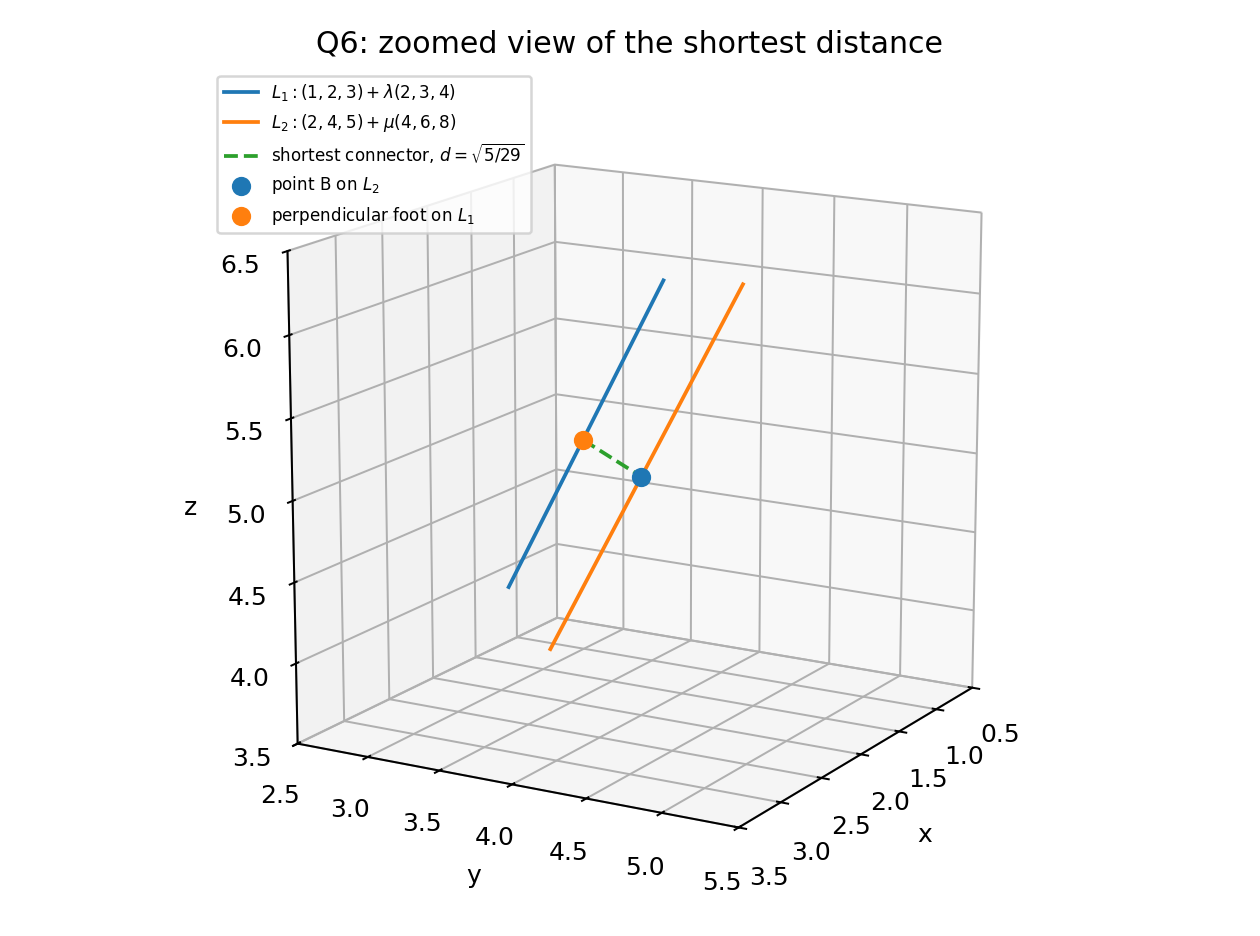
\includegraphics[width=0.96\linewidth]{figs/C12/Q06.png}\end{figure}
\par\smallskip\noindent\textbf{Code reference -}\par\noindent\fbox{\parbox{\dimexpr\linewidth-2\fboxsep-2\fboxrule\relax}{\centering\texttt{codes/C12/Q06.py}}}

\paragraph*{Lines and planes}
\item \label{question:C12-Q10}\label{question-short:C12-Q10} Find the plane through the intersection of $2x+y-z=3$ and $5x-3y+4z+9=0$ that is parallel to $\frac{x-1}{2}=\frac{y-3}{-4}=\frac{5-z}{-5}$.
\engsolution
Let
\formulausedplain{P_1=2x+y-z-3.}
\formulausedplain{P_2=5x-3y+4z+9.}
Every plane through the intersection line belongs to the affine pencil $P_1+\lambda P_2=0$. Its normal is
\formulausedplain{
\vec n(\lambda)=(2+5\lambda,\,1-3\lambda,\,-1+4\lambda).
}
The direction of the given line is $\vec d=(2,-4,5)$. The required parallelism condition is
\formulaused{(\vec n_1+\lambda\vec n_2)\cdot\vec d=0.}{C12-Q10}
Substitution gives
\formulausedplain{
2(2+5\lambda)-4(1-3\lambda)+5(-1+4\lambda)=0,
}
so $-5+42\lambda=0$ and $\lambda=5/42$. Multiplying the pencil by 42 yields
\formulausedplain{
42P_1+5P_2=0
\Longrightarrow 109x+27y-22z-81=0.
}
The plane contains the intersection line by construction, and its normal has zero dot product with the given line direction.
\begin{figure}[H]\centering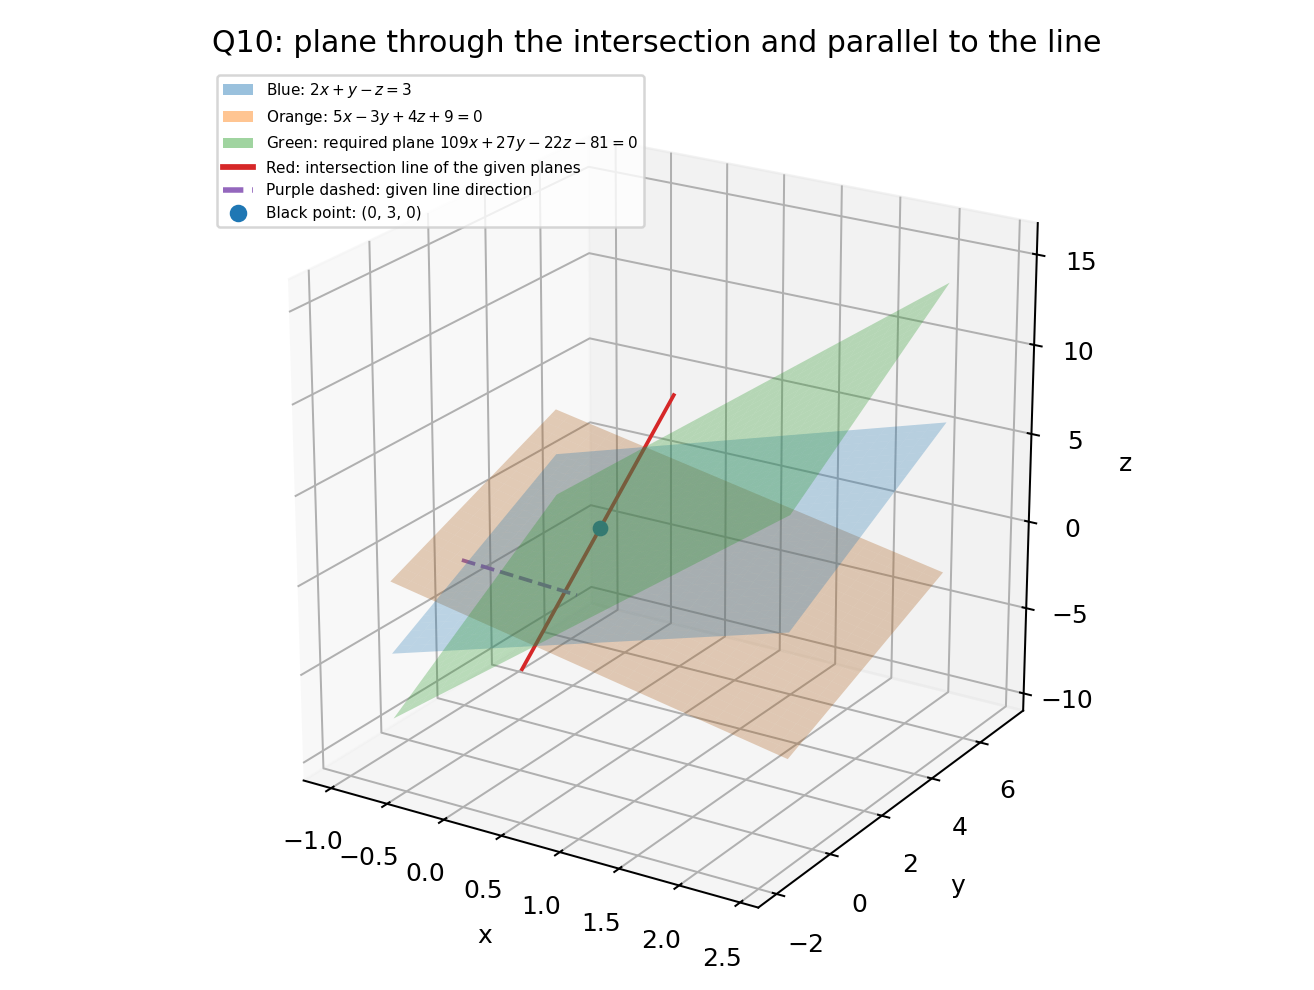
\includegraphics[width=0.96\linewidth]{figs/C12/Q10.png}\end{figure}
\par\smallskip\noindent\textbf{Code reference -}\par\noindent\fbox{\parbox{\dimexpr\linewidth-2\fboxsep-2\fboxrule\relax}{\centering\texttt{codes/C12/Q10.py}}}

\item \label{question:C12-Q15}\label{question-short:C12-Q15} Find where the line through $A(3,4,1)$ and $B(5,1,6)$ meets the plane through $P(2,1,2)$, $Q(3,1,0)$ and $R(4,-2,1)$.
\engsolution
The two plane-edge vectors are
\formulausedplain{Q-P=(1,0,-2).}
\formulausedplain{R-P=(2,-3,-1).}
Their cross product is proportional to $(2,1,1)$, so the plane equation is
\formulausedplain{
2(x-2)+(y-1)+(z-2)=0
\Longrightarrow 2x+y+z=7.
}
The line direction is $B-A=(2,-3,5)$. Its affine representation is
\formulaused{\vec r=\vec A+t\vec d.}{C12-Q15}
Thus
\formulausedplain{
\vec r=(3,4,1)+t(2,-3,5).
}
Substitution into the plane gives
\formulausedplain{
2(3+2t)+(4-3t)+(1+5t)=7
\Longrightarrow 11+6t=7
\Longrightarrow t=-\frac23.
}
The intersection point is therefore
\formulausedplain{
\left(\frac53,6,-\frac73\right).
}
Putting this point back into $2x+y+z$ gives $10/3+6-7/3=7$, which verifies the incidence condition.
\begin{figure}[H]\centering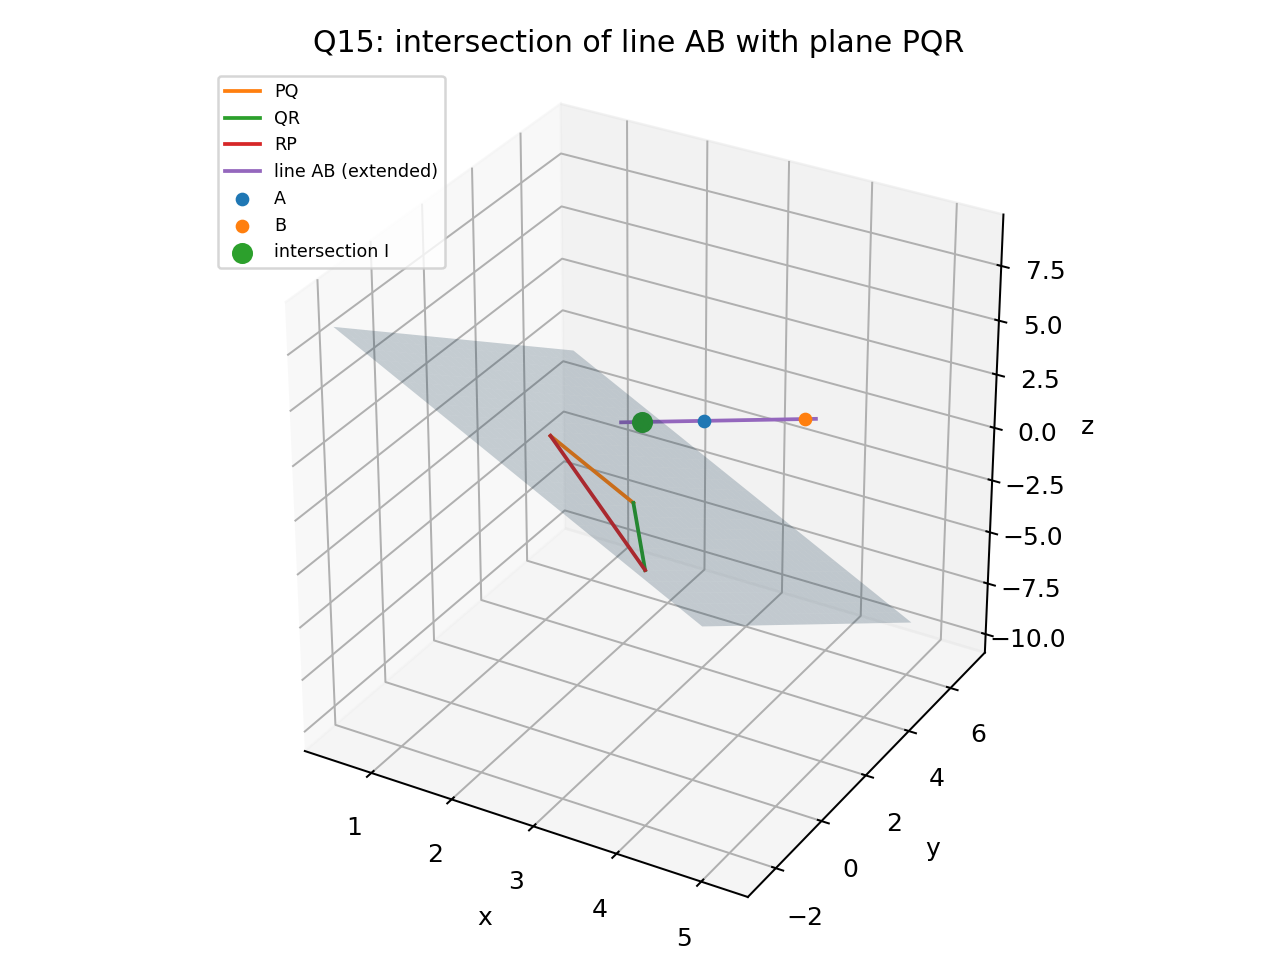
\includegraphics[width=0.96\linewidth]{figs/C12/Q15.png}\end{figure}
\par\smallskip\noindent\textbf{Code reference -}\par\noindent\fbox{\parbox{\dimexpr\linewidth-2\fboxsep-2\fboxrule\relax}{\centering\texttt{codes/C12/Q15.py}}}

\item \label{question:C12-Q25}\label{question-short:C12-Q25} If $y=\log\left(\frac{x}{a+bx}\right)^x$, prove that $x^3y''=(xy'-y)^2$.
\engsolution
Interpret the displayed power as
\formulausedplain{
y=x\log\left(\frac{x}{a+bx}\right),
}
on a domain where the logarithm is defined. The logarithmic derivative identity and the Euler operator $\theta=x\,d/dx$ give
\formulaused{\frac{d}{dx}\log|u|=\frac{u'}u.}{C12-Q25}
\formulaused{\theta y-y=xy'-y}{C12-Q25-S01}
Differentiate $y$ explicitly:
\formulausedplain{
y'=\log\left(\frac{x}{a+bx}\right)+x\left(\frac1x-\frac b{a+bx}\right)
=\log\left(\frac{x}{a+bx}\right)+\frac a{a+bx}.
}
Differentiating once more,
\formulausedplain{
y''=\frac1x-\frac b{a+bx}-\frac{ab}{(a+bx)^2}
=\frac{a^2}{x(a+bx)^2}.
}
The Euler combination simplifies without the logarithm:
\formulausedplain{
xy'-y=x\frac a{a+bx}=\frac{ax}{a+bx}.
}
Squaring it and comparing with $y''$ gives
\formulausedplain{
(xy'-y)^2=\frac{a^2x^2}{(a+bx)^2}=x^3\frac{a^2}{x(a+bx)^2}=x^3y''.
}
Hence
\formulausedplain{
x^3y''=(xy'-y)^2.
}

\paragraph*{Matrices and determinants}
\item \label{question:C12-Q28}\label{question-short:C12-Q28} If $A=\myvec{\cos\theta&\sin\theta\\\sin\theta&\cos\theta}$, find $\det(A^n)$ for natural $n$.
\engsolution
The symmetric matrix has eigenvectors $q_+=(1,1)^T$ and $q_-=(1,-1)^T$. Their eigenvalues are
\formulausedplain{\lambda_+=\cos\theta+\sin\theta.}
\formulausedplain{\lambda_-=\cos\theta-\sin\theta.}
Spectral decomposition therefore gives $\det A=\lambda_+\lambda_-$ and raises each eigenvalue to the $n$th power. Using the determinant-power identity,
\formulaused{\det(A^n)=(\det A)^n.}{C12-Q28}
We obtain
\formulausedplain{
\det(A^n)=(\lambda_+\lambda_-)^n
=\bigl((\cos\theta+\sin\theta)(\cos\theta-\sin\theta)\bigr)^n
=(\cos2\theta)^n.
}

\item \label{question:C12-Q30}\label{question-short:C12-Q30} Find the inverse of $\myvec{0&1&2\\1&2&3\\3&1&0}$ using elementary row operations.
\engsolution
Let
\formulausedplain{
A=\myvec{0&1&2\\1&2&3\\3&1&0}.
}
Swap the first two rows to obtain a unit pivot, then eliminate below the pivots. The exact factorization is
\formulausedplain{PA=LU.}
\formulausedplain{L=\myvec{1&0&0\\0&1&0\\3&-5&1}.}
\formulausedplain{U=\myvec{1&2&3\\0&1&2\\0&0&1}.}
The inverse is the matrix $X$ satisfying $AX=I$; this defining relation is
\formulaused{AA^{-1}=I.}{C12-Q30}
Solving the three triangular systems for the columns of $X$ gives
\formulausedplain{
A^{-1}=\myvec{3&-2&1\\-9&6&-2\\5&-3&1}.
}
For the consistency check, multiplication of the first row gives $(0,1,2)A^{-1}=(1,0,0)$, and the other two rows similarly give $(0,1,0)$ and $(0,0,1)$. Therefore
\[
A^{-1}=\myvec{3&-2&1\\-9&6&-2\\5&-3&1}.
\]
\par\smallskip\noindent\textbf{Code reference -}\par\noindent\fbox{\parbox{\dimexpr\linewidth-2\fboxsep-2\fboxrule\relax}{\centering\texttt{codes/C12/Q30.py}}}

\item \label{question:C12-Q36}\label{question-short:C12-Q36} If $a+b+c\ne0$ and $\mydet{a&b&c\\b&c&a\\c&a&b}=0$, prove that $a=b=c$.
\engsolution
Let $A$ be the cyclic matrix in the question and let $\omega=e^{-2\pi i/3}$, so $1+\omega+\omega^2=0$. The three-point DFT basis diagonalizes $A$, with eigenvalues
\formulaused{\lambda_0=a+b+c.}{C12-Q36-F01}
\formulaused{\lambda_1=a+b\omega+c\omega^2.}{C12-Q36-F01-S01}
\formulaused{\lambda_2=a+b\omega^2+c\omega.}{C12-Q36-F01-S02}
The determinant factorization is
\formulaused{
0=\det A=-\lambda_0\lambda_1\lambda_2
=-(a+b+c)(a^2+b^2+c^2-ab-bc-ca).
}{C12-Q36-F02}
Because $a+b+c\ne0$, the second factor must vanish. The required sum-of-squares identity is
\formulaused{a^2+b^2+c^2-ab-bc-ca=\frac12\bigl((a-b)^2+(b-c)^2+(c-a)^2\bigr).}{C12-Q36}
For real $a,b,c$, each square is nonnegative. Their sum can be zero only if
\formulausedplain{
a-b=0,\qquad b-c=0,\qquad c-a=0.
}
Hence
\formulausedplain{
a=b=c.
}

\item \label{question:C12-Q48}\label{question-short:C12-Q48} Discuss continuity and differentiability of $f(x)=|x|+|x-1|$ on $(-1,2)$.
\engsolution
The absolute-value characteristic changes branch at $x=0$ and $x=1$. Resolving the signs gives
\formulausedplain{f(x)=|x|+|x-1|=\begin{cases}1-2x,&-1<x<0,\\1,&0\le x<1,\\2x-1,&1\le x<2.\end{cases}}
At the first breakpoint,
\formulausedplain{
\lim_{x\to0^-}f(x)=1=f(0)=\lim_{x\to0^+}f(x),
}
and at the second,
\formulausedplain{
\lim_{x\to1^-}f(x)=1=f(1)=\lim_{x\to1^+}f(x).
}
Thus the function is continuous throughout $(-1,2)$. Its one-sided derivatives are
\formulausedplain{f'_-(0)=-2.}
\formulausedplain{f'_+(0)=0.}
\formulausedplain{f'_-(1)=0.}
\formulausedplain{f'_+(1)=2.}
The slopes disagree at both breakpoints, so $f$ is not differentiable at $0$ or $1$, but is differentiable elsewhere. Every branch has slope magnitude at most $2$, hence the piecewise map is Lipschitz with constant $2$.
\begin{figure}[H]\centering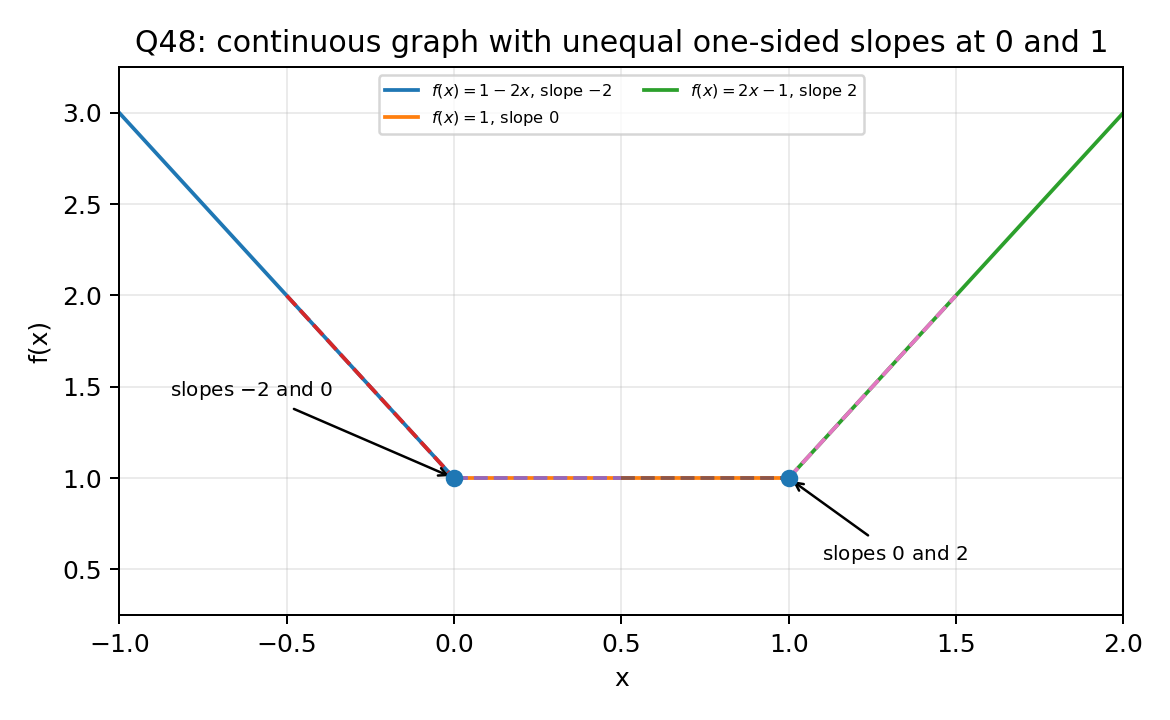
\includegraphics[width=0.92\linewidth]{figs/C12/Q48.png}\end{figure}
\par\smallskip\noindent\textbf{Code reference -}\par\noindent\fbox{\parbox{\dimexpr\linewidth-2\fboxsep-2\fboxrule\relax}{\centering\texttt{codes/C12/Q48.py}}}

\item \label{question:C12-Q49}\label{question-short:C12-Q49} On $\mathbb R$, define $(a,b)\in R$ when $a-b+\sqrt3$ is irrational. Determine whether $R$ is reflexive, symmetric and transitive.
\engsolution
Write the relation as the predicate $R(a,b)$: the number $a-b+\sqrt3$ must lie outside $\mathbb Q$. Its defining condition is
\formulausedplain{R(a,b)\Longleftrightarrow a-b+\sqrt3\text{ is irrational}.}
For reflexivity, $a-a+\sqrt3=\sqrt3$ is irrational, so $R(a,a)$ holds for every $a$. Symmetry fails: with $(a,b)=(\sqrt3,0)$, the forward expression is $2\sqrt3$ (irrational), but the reversed expression is $0$ (rational). Transitivity fails for
\formulausedplain{a=0.}
\formulausedplain{b=\frac{\sqrt3}{2}.}
\formulausedplain{c=\sqrt3.}
Both $a-b+\sqrt3=\sqrt3/2$ and $b-c+\sqrt3=\sqrt3/2$ are irrational, while $a-c+\sqrt3=0$. Therefore
\formulausedplain{
R\text{ is reflexive, but neither symmetric nor transitive}.
}

\paragraph*{Algebraic structures}
\item \label{question:C12-Q50}\label{question-short:C12-Q50} On $\mathbb R\times\mathbb R$, define $(a,b)*(c,d)=(a+c,b+d)$. Prove commutativity and associativity, and find the identity and the inverse of $(3,-5)$.
\engsolution
The operation is coordinatewise addition, so it is closed on $\mathbb R^2$. Its defining law is
\formulaused{(a,b)*(c,d)=(a+c,b+d).}{C12-Q50}
For associativity,
\formulaused{
((a,b)*(c,d))*(e,f)=(a+c+e,b+d+f)
=(a,b)*((c,d)*(e,f)).
}{C12-Q50-F01}
For commutativity,
\formulaused{
(a,b)*(c,d)=(a+c,b+d)=(c+a,d+b)=(c,d)*(a,b).
}{C12-Q50-F02}
The identity is $(0,0)$, and the inverse of $(3,-5)$ solves
\formulausedplain{
(3,-5)*(u,v)=(3+u,-5+v)=(0,0),
}
so it is $(-3,5)$. Thus the structure is an Abelian group and
\formulausedplain{
e=(0,0),\qquad (3,-5)^{-1}=(-3,5).
}

\item \label{question:C12-Q51}\label{question-short:C12-Q51} On $\{0,1,2,3,4,5,6\}$ define $a*b=a+b$ if $a+b<7$, and $a*b=a+b-7$ otherwise. Give the operation table and show that 0 is the identity and $7-a$ is the inverse for nonzero $a$.
\engsolution
The piecewise definition is addition modulo $7$:
\formulaused{a*b=(a+b)\bmod 7.}{C12-Q51}
The Cayley table is
\formulausedplain{
\begin{array}{c|rrrrrrr}* &0&1&2&3&4&5&6\\\hline
0&0&1&2&3&4&5&6\\1&1&2&3&4&5&6&0\\2&2&3&4&5&6&0&1\\3&3&4&5&6&0&1&2\\4&4&5&6&0&1&2&3\\5&5&6&0&1&2&3&4\\6&6&0&1&2&3&4&5
\end{array}
}
The first row and column show $0*a=a*0=a$. For nonzero $a$, the residue $7-a$ lies in the set and
\formulaused{
a*(7-a)=a+7-a\equiv0\pmod7.
}{C12-Q51-F02}
Since $7$ is prime, every nonzero residue generates the cyclic group $\mathbb Z_7$. Therefore
\formulausedplain{
0\text{ is the identity and }a^{-1}=7-a\pmod7.
}

\item \label{question:C12-Q52}\label{question-short:C12-Q52} Find any point of discontinuity of $f(x)=x-|x-x^2|$, $x\in[-1,1]$.
\engsolution
Factor the expression inside the absolute value:
\formulaused{
x-x^2=x(1-x).
}{C12-Q52}
On $[-1,1]$, this quantity is nonnegative for $0\le x\le1$ and nonpositive for $-1\le x\le0$. The piecewise nonlinear map is therefore
\formulausedplain{f(x)=\begin{cases}2x-x^2,&-1\le x\le0,\\x^2,&0\le x\le1.\end{cases}}
At the switching point, both branches give $f(0)=0$. Moreover,
\formulausedplain{
\lim_{x\to0^-}(2x-x^2)=0=f(0)=\lim_{x\to0^+}x^2.
}
Thus there is no discontinuity on the domain. The branch derivatives $2-2x$ and $2x$ are bounded in magnitude by $4$, providing the stated Lipschitz consistency check. Hence
\formulausedplain{
\text{there is no point of discontinuity on }[-1,1].
}
\begin{figure}[H]\centering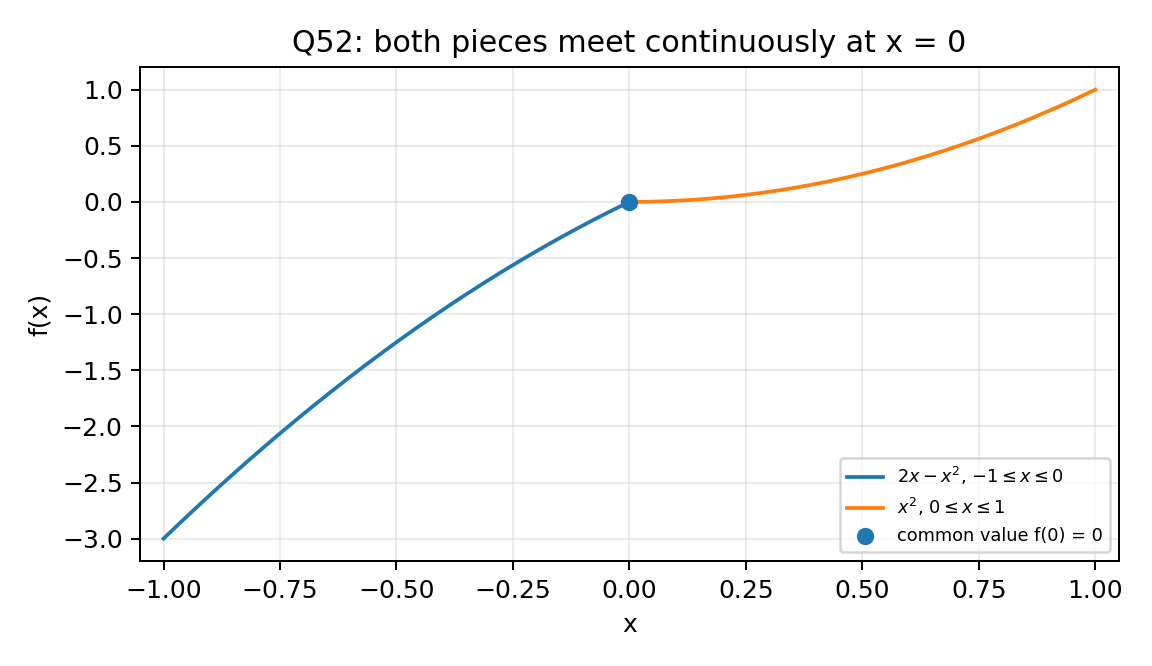
\includegraphics[width=0.92\linewidth]{figs/C12/Q52.png}\end{figure}
\par\smallskip\noindent\textbf{Code reference -}\par\noindent\fbox{\parbox{\dimexpr\linewidth-2\fboxsep-2\fboxrule\relax}{\centering\texttt{codes/C12/Q52.py}}}

\item \label{question:C12-Q53}\label{question-short:C12-Q53} A man steps forward with probability $0.4$ and backward with probability $0.6$. Find the probability that after 5 steps he is one step away from his starting point.
\engsolution
Encode a forward step by $z$ and a backward step by $z^{-1}$. The one-step bilateral Laurent PGF and its five-step product are
\formulausedplain{G_5(z)=(0.4z+0.6z^{-1})^5.}
After five steps, displacement $+1$ requires three forward and two backward steps, while displacement $-1$ requires two forward and three backward steps. Extracting the two Laurent coefficients gives
\formulausedplain{
P(|D|=1)=\binom53(0.4)^3(0.6)^2+\binom52(0.4)^2(0.6)^3.
}
Numerically,
\formulausedplain{
\binom53(0.064)(0.36)+\binom52(0.16)(0.216)
=0.3456+0.2304=0.576.
}
The two cases are disjoint and exhaust the requested one-step displacement events.
\begin{figure}[H]\centering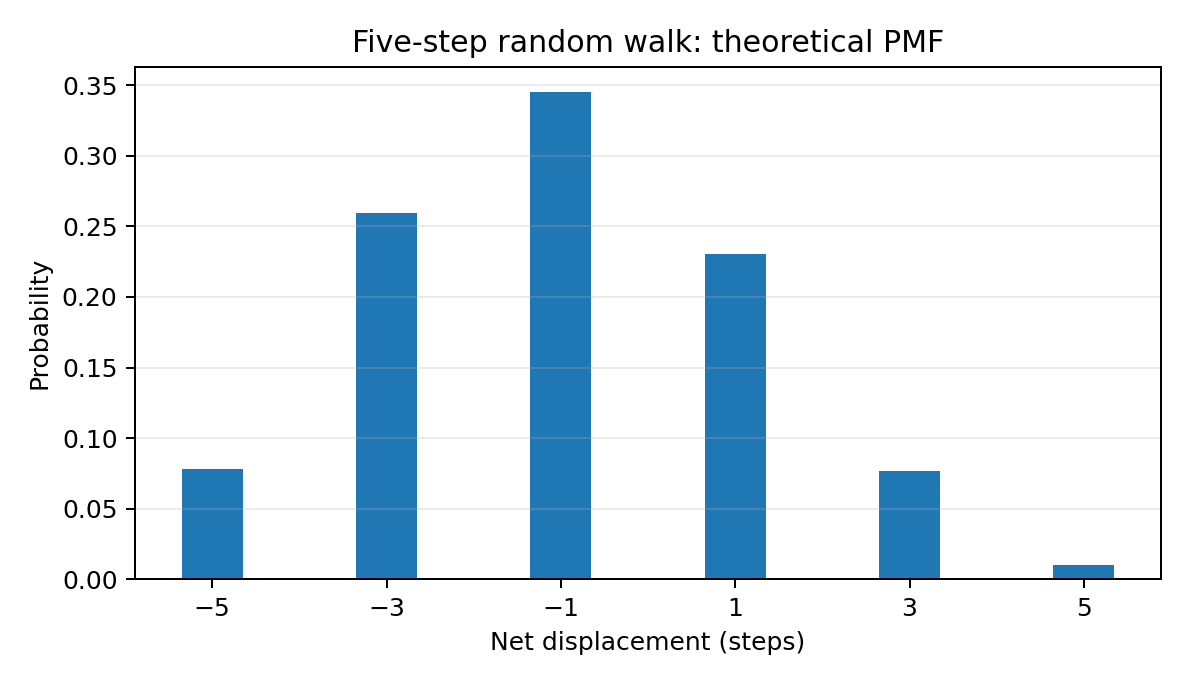
\includegraphics[width=0.92\linewidth]{figs/C12/Q53.png}\end{figure}
\par\smallskip\noindent\textbf{Code reference -}\par\noindent\fbox{\parbox{\dimexpr\linewidth-2\fboxsep-2\fboxrule\relax}{\centering\texttt{codes/C12/Q53.py}}}

\item \label{question:C12-Q54}\label{question-short:C12-Q54} A girl throws a die. If it shows 1 or 2, she tosses a coin three times; otherwise she tosses it once. Given that exactly one tail was obtained, find the probability that the die showed 3, 4, 5 or 6.
\engsolution
Let $H_1$ denote die outcomes $1$ or $2$, $H_2$ denote outcomes $3,4,5,6$, and let $E$ be the event of exactly one tail. Then
\formulausedplain{P(H_1)=\frac13.}
\formulausedplain{P(H_2)=\frac23.}
Under $H_1$, exactly one tail in three tosses has likelihood $3(1/2)^3=3/8$; under $H_2$, exactly one tail in one toss has likelihood $1/2$. Bayes' rule is
\formulaused{P(H_2\mid E)=\frac{P(E\mid H_2)P(H_2)}{P(E)}.}{C12-Q54}
The evidence probability is
\formulausedplain{
P(E)=\frac38\cdot\frac13+\frac12\cdot\frac23=\frac18+\frac13=\frac{11}{24}.
}
Therefore
\formulausedplain{
P(H_2\mid E)=\frac{(1/2)(2/3)}{11/24}=\frac{1/3}{11/24}=\frac8{11}.
}

\item \label{question:C12-Q55}\label{question-short:C12-Q55} An urn contains 5 red and 2 black balls. Two balls are drawn without replacement. Let $X$ be the number of black balls. State its possible values and find its mean and variance.
\engsolution
Without replacement, $X$ has a hypergeometric distribution with population size $N=7$, black count $K=2$, and sample size $n=2$. Thus $X\in\{0,1,2\}$ and the probability mass is
\formulausedplain{P(X=0)=\frac{10}{21}.}
\formulausedplain{P(X=1)=\frac{10}{21}.}
\formulausedplain{P(X=2)=\frac1{21}.}
The three probabilities are
\formulausedplain{
P(X=0)=\frac{10}{21},\qquad P(X=1)=\frac{10}{21},\qquad P(X=2)=\frac1{21}.
}
The probability-generating function method uses
\formulaused{G_X(z)=\sum_xP(X=x)z^x.}{C12-Q55}
Here
\formulausedplain{G_X(z)=\frac{10+10z+z^2}{21}.}
\formulausedplain{G'_X(1)=\frac{12}{21}=\frac47.}
and
\formulausedplain{
G''_X(1)=\frac2{21}=E[X(X-1)].
}
Consequently,
\formulausedplain{
E[X^2]=E[X(X-1)]+E[X]=\frac2{21}+\frac47=\frac{20}{21},
}
\formulausedplain{
\operatorname{Var}(X)=E[X^2]-E[X]^2=\frac{20}{21}-\frac{16}{49}=\frac{50}{147}.
}
\begin{figure}[H]\centering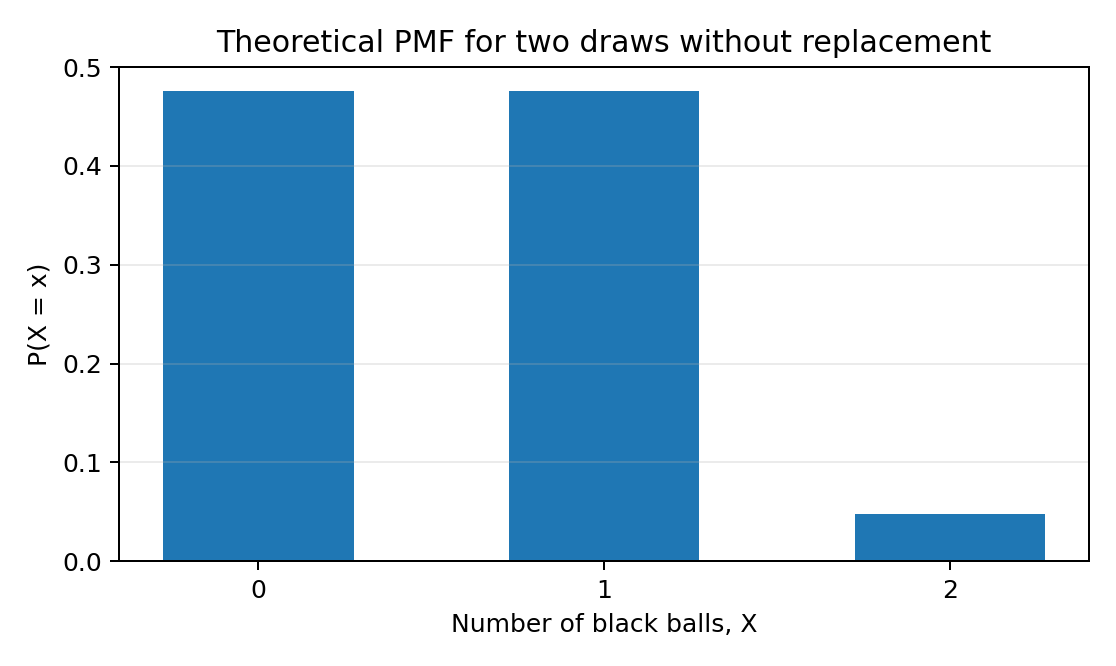
\includegraphics[width=0.92\linewidth]{figs/C12/Q55.png}\end{figure}
\par\smallskip\noindent\textbf{Code reference -}\par\noindent\fbox{\parbox{\dimexpr\linewidth-2\fboxsep-2\fboxrule\relax}{\centering\texttt{codes/C12/Q55.py}}}

\item \label{question:C12-Q56}\label{question-short:C12-Q56} In 3 trials of a binomial distribution, the probability of exactly 2 successes is 9 times the probability of 3 successes. Find the success probability.
\engsolution
For three independent trials with success probability $p$, the binomial PGF is
\formulaused{G(z)=(1-p+pz)^3.}{C12-Q56}
The coefficients of $z^2$ and $z^3$ are
\formulausedplain{P(X=2)=\binom32p^2(1-p)=3p^2(1-p).}
\formulausedplain{P(X=3)=p^3.}
The given relation produces
\formulausedplain{
3p^2(1-p)=9p^3
\Longrightarrow 3p^2(1-4p)=0.
}
Both roots are admissible probabilities in $[0,1]$:
\formulausedplain{
p=0\quad\text{or}\quad p=\frac14.
}
The $p=0$ case makes both probabilities zero, so it is retained as an edge case rather than divided away.
\par\smallskip\noindent\textbf{Code reference -}\par\noindent\fbox{\parbox{\dimexpr\linewidth-2\fboxsep-2\fboxrule\relax}{\centering\texttt{codes/C12/Q56.py}}}

\item \label{question:C12-Q57}\label{question-short:C12-Q57} An urn contains 3 red and 5 black balls. A ball is drawn, its colour recorded and returned, and 2 more balls of that colour are added. Then two balls are drawn without replacement. Find the probability both are red.
\engsolution
Condition on the colour of the reinforced first draw. The initial state is $(R,B)=(3,5)$, so the branch probabilities are $3/8$ and $5/8$. After a red first draw the state is $(5,5)$; after a black first draw it is $(3,7)$. The law of total probability is
\formulaused{P(E)=\sum_iP(E\mid S_i)P(S_i).}{C12-Q57}
For the red branch,
\formulausedplain{
P(RR\mid R_1)=\frac5{10}\frac4{9}=\frac29.
}
For the black branch,
\formulausedplain{
P(RR\mid B_1)=\frac3{10}\frac2{9}=\frac1{15}.
}
Combining the mutually exclusive branches,
\formulausedplain{
P(RR)=\frac38\frac29+\frac58\frac1{15}
=\frac1{12}+\frac1{24}=\frac18.
}
The state update is applied before the two final draws, preserving the reinforcement dependence.
\par\smallskip\noindent\textbf{Code reference -}\par\noindent\fbox{\parbox{\dimexpr\linewidth-2\fboxsep-2\fboxrule\relax}{\centering\texttt{codes/C12/Q57.py}}}

\paragraph*{Optimization}
\item \label{question:C12-Q59}\label{question-short:C12-Q59} Solve graphically: minimise $z=3x+5y$ subject to $x+2y\ge10$, $x+y\ge6$, $3x+y\ge8$, $x,y\ge0$.
\engsolution
The feasible region is the intersection of three half-planes in the first quadrant. Its relevant corner is obtained by making the first two constraints active:
\formulausedplain{x+2y=10.}
\formulausedplain{x+y=6.}
The objective admits the duality decomposition
\formulausedplain{3x+5y=2(x+2y)+(x+y).}
For every feasible point this gives $3x+5y\ge2(10)+6=26$. At $(2,4)$ equality holds, and the third constraint is satisfied because $3(2)+4=10\ge8$. Therefore the graphical minimum is
\formulausedplain{
(x,y)=(2,4),\qquad z_{\min}=3(2)+5(4)=26.
}
Equivalently, the dual certificate $(u,v,w)=(2,1,0)$ is feasible and has objective value $20+6=26$, confirming global optimality.
\begin{figure}[H]\centering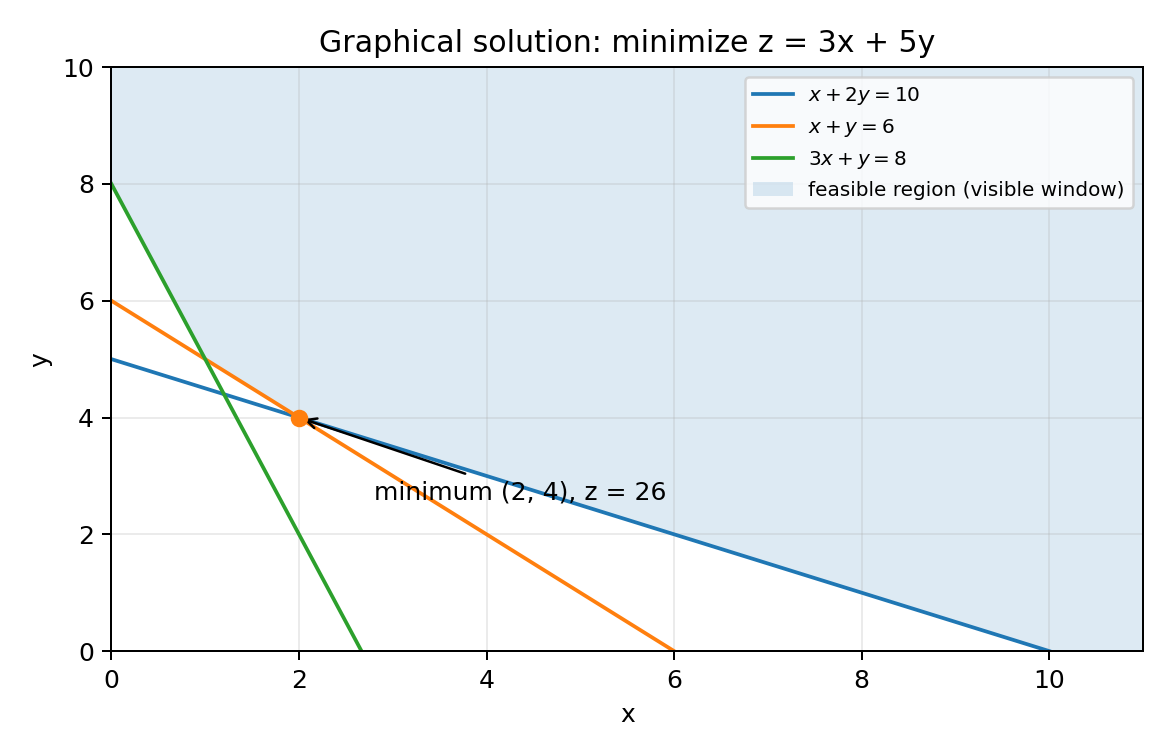
\includegraphics[width=0.92\linewidth]{figs/C12/Q59.png}\end{figure}
\par\smallskip\noindent\textbf{Code reference -}\par\noindent\fbox{\parbox{\dimexpr\linewidth-2\fboxsep-2\fboxrule\relax}{\centering\texttt{codes/C12/Q59.py}}}

\item \label{question:C12-Q60}\label{question-short:C12-Q60} A dealer has Rs. 57,600 and space for at most 20 sewing machines. An electronic machine costs Rs. 3600 and earns Rs. 220 profit; a manual machine costs Rs. 2400 and earns Rs. 180 profit. How should he invest to maximise profit?
\engsolution
Let $e$ and $m$ be the numbers of electronic and manual machines. Divide the budget constraint by Rs. 1200 to obtain
\formulausedplain{3e+2m\le48.}
\formulausedplain{e+m\le20.}
\formulausedplain{e,m\ge0.}
The primal objective is $P=220e+180m$. The complementary-slackness equations for a tight optimum are
\formulausedplain{3u+v=220.}
\formulausedplain{2u+v=180.}
Subtracting gives $u=40$, and then $v=100$. The dual value is
\formulausedplain{
48u+20v=48(40)+20(100)=3920.
}
The primal intersection of the two resource boundaries satisfies
\formulausedplain{
3e+2m=48,\qquad e+m=20
\Longrightarrow e=8,\quad m=12.
}
Its profit is
\formulausedplain{3e+2m=48.}
\formulausedplain{e+m=20.}
Both resource constraints are tight, and primal and dual values agree, so complementary slackness certifies the allocation $(e,m)=(8,12)$.
\begin{figure}[H]\centering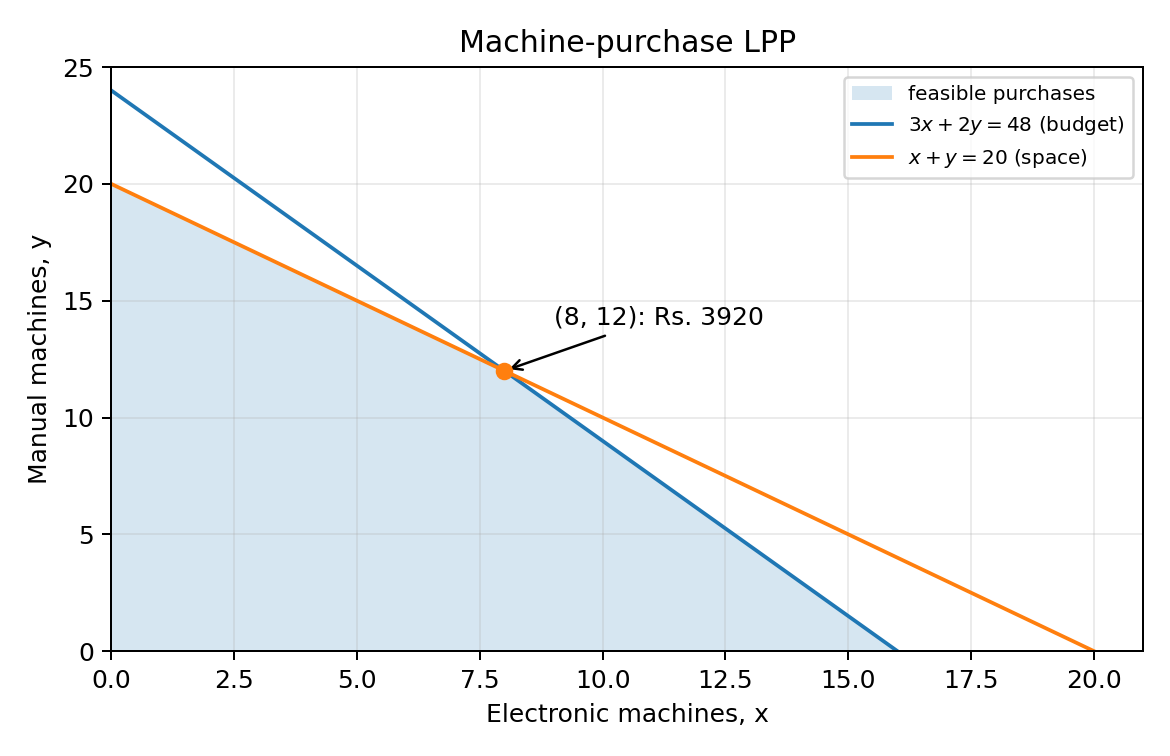
\includegraphics[width=0.92\linewidth]{figs/C12/Q60.png}\end{figure}
\par\smallskip\noindent\textbf{Code reference -}\par\noindent\fbox{\parbox{\dimexpr\linewidth-2\fboxsep-2\fboxrule\relax}{\centering\texttt{codes/C12/Q60.py}}}

\item \label{question:C12-Q64}\label{question-short:C12-Q64} A tangent to $x^2+y^2=4$ at a point in the first quadrant meets the positive axes at $A$ and $B$. Find the minimum of $OA+OB$.
\engsolution
Parameterize the point of tangency by $(2\cos\theta,2\sin\theta)$ with $0<\theta<\pi/2$. The tangent and its intercepts follow from the constrained geometry:
\formulausedplain{\tan\theta:\quad x\cos\theta+y\sin\theta=2.}
Setting $y=0$ and $x=0$ gives intercept lengths $OA=2\sec\theta$ and $OB=2\csc\theta$. Hence
\formulausedplain{
F(\theta)=OA+OB=2\sec\theta+2\csc\theta.
}
Stationarity gives
\formulausedplain{
F'(\theta)=2\sec\theta\tan\theta-2\csc\theta\cot\theta=0.
}
After multiplying by positive factors in the first quadrant,
\formulausedplain{
\sin^3\theta=\cos^3\theta\Longrightarrow \theta=\frac\pi4.
}
The objective tends to infinity at either open endpoint, so this stationary point is the global minimum. Therefore
\formulausedplain{
F_{\min}=2\sqrt2+2\sqrt2=4\sqrt2.
}
\begin{figure}[H]\centering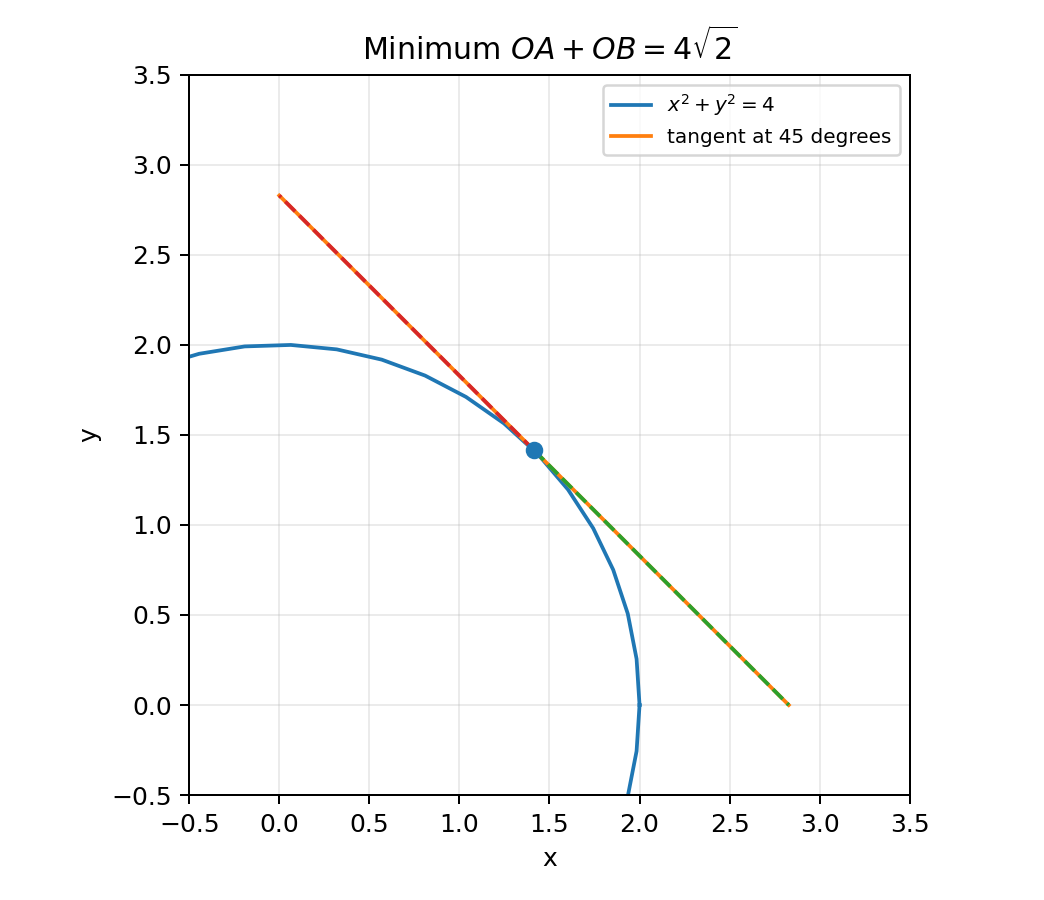
\includegraphics[width=0.92\linewidth]{figs/C12/Q64.png}\end{figure}
\par\smallskip\noindent\textbf{Code reference -}\par\noindent\fbox{\parbox{\dimexpr\linewidth-2\fboxsep-2\fboxrule\relax}{\centering\texttt{codes/C12/Q64.py}}}

\item \label{question:C12-Q65}\label{question-short:C12-Q65} Find the maximum area of an isosceles triangle inscribed in $\frac{x^2}{16}+\frac{y^2}{9}=1$ with its vertex at an end of the major axis.
\engsolution
Fix the vertex at $(4,0)$ and use symmetry for the base points:
\formulausedplain{P=(u,v).}
\formulausedplain{Q=(u,-v).}
The ellipse constraint gives $v=3\sqrt{1-u^2/16}$, with $-4\le u\le4$. The base has length $2v$ and the horizontal altitude is $4-u$, so the constrained area objective is
\formulausedplain{A(u)=3(4-u)\sqrt{1-u^2/16},\qquad -4\le u\le4.}
To locate interior extrema, maximize the square of the nonnegative area. Differentiating the equivalent expression
\formulausedplain{
A(u)^2=9(4-u)^2\left(1-\frac{u^2}{16}\right)
}
gives the stationary condition $u=-2$ (the other factor corresponds to a zero-area endpoint). The endpoints $u=\pm4$ give $A=0$, while at the interior point
\formulausedplain{
A(-2)=3(4+2)\sqrt{1-\frac4{16}}
=18\sqrt{\frac34}=9\sqrt3.
}
Since the feasible interval is compact and the endpoints have zero area, this positive stationary value is the global maximum.
\begin{figure}[H]\centering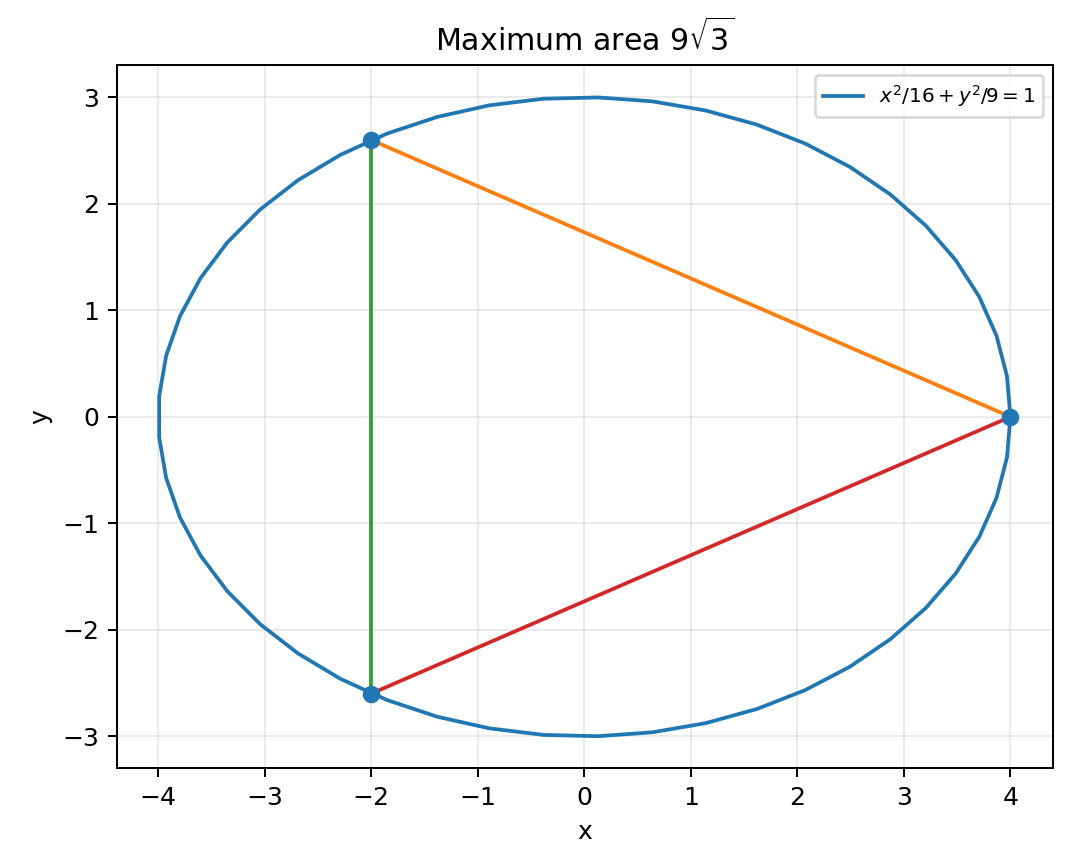
\includegraphics[width=0.92\linewidth]{figs/C12/Q65.png}\end{figure}
\par\smallskip\noindent\textbf{Code reference -}\par\noindent\fbox{\parbox{\dimexpr\linewidth-2\fboxsep-2\fboxrule\relax}{\centering\texttt{codes/C12/Q65.py}}}
\end{enumerate}


